\documentclass[12pt,a4paper]{article}

\usepackage[top=2.5cm,bottom=2.5cm,left=2.7cm,right=2.7cm]{geometry}
\usepackage[T1]{fontenc}
\usepackage[utf8]{inputenc}
\usepackage{lmodern}
\usepackage{microtype}
\usepackage{booktabs}
\usepackage{longtable}
\usepackage{array}
\usepackage{tabularx}
\usepackage{ragged2e}
\usepackage{enumitem}
\usepackage{xcolor}
\usepackage{hyperref}
\usepackage{fancyhdr}
\usepackage{titlesec}
\usepackage{parskip}
\usepackage{float}
\usepackage{colortbl}
\usepackage{graphicx}
\usepackage{tikz}
\usetikzlibrary{positioning, arrows.meta, fit, backgrounds, calc, shapes.geometric, shapes.multipart}

\definecolor{headerblue}{RGB}{20,62,128}
\definecolor{textgray}{RGB}{75,75,75}
\definecolor{accent}{RGB}{32,113,167}
\definecolor{rowlight}{RGB}{237,244,252}
\definecolor{rowwhite}{RGB}{255,255,255}
\definecolor{modcms}{RGB}{52,152,219}
\definecolor{modscholar}{RGB}{46,204,113}
\definecolor{modevents}{RGB}{231,76,60}
\definecolor{modvenue}{RGB}{155,89,182}
\definecolor{modsystem}{RGB}{241,196,15}

\renewcommand{\arraystretch}{1.35}
\hypersetup{
  colorlinks=true,
  linkcolor=headerblue,
  urlcolor=accent,
  pdftitle={System Design Document - Digital Department Hub},
  pdfauthor={du\_vagabond}
}

\pagestyle{fancy}
\fancyhf{}
\lhead{\small\color{textgray}SDD v1.1 | Digital Department Hub}
\rhead{\small\color{textgray}CMS, Events, Scholarships, and Resource Booking}
\cfoot{\thepage}
\renewcommand{\headrulewidth}{0.4pt}
\setlength{\headheight}{14.5pt}

\titleformat{\section}
  {\large\bfseries\color{headerblue}}
  {\thesection}{0.75em}{}[\vspace{-4pt}\rule{\linewidth}{0.5pt}]
\titleformat{\subsection}
  {\normalsize\bfseries\color{textgray}}
  {\thesubsection}{0.6em}{}

\newcolumntype{L}[1]{>{\RaggedRight\arraybackslash}p{#1}}
\newcolumntype{C}[1]{>{\Centering\arraybackslash}p{#1}}
\newcolumntype{Y}{>{\RaggedRight\arraybackslash}X}
\newcommand{\thead}[1]{\textbf{\color{white}#1}}
\newcommand{\theadrow}{\rowcolor{headerblue}}

\begin{document}

\pagenumbering{gobble}
\begin{titlepage}
\centering
\vspace*{0.3cm}

\IfFileExists{logo.png}{%
  
\includegraphics[width=2.8cm]{logo.png}%
}{%
  \fbox{\begin{minipage}[c][2.8cm][c]{2.8cm}\centering\textbf{Logo}\\\texttt{logo.png}\end{minipage}}%
}
\par\vspace{0.2cm}
{\Large\bfseries University of Dhaka\par}
\vspace{0.15cm}
{\large Department of Computer Science and Engineering\par}

\vspace{0.6cm}
{\Huge\bfseries\color{headerblue}System Design Document\par}
\vspace{0.3cm}
{\LARGE\bfseries Digital Department Hub\par}
\vspace{0.15cm}
{\large CMS, Events, Scholarships, and Resource Booking\par}
\vspace{0.5cm}
\rule{0.82\textwidth}{1pt}\par
\vspace{0.35cm}
{\renewcommand{\arraystretch}{1.15}%
\begin{tabular}{@{}ll@{}}
\textbf{Course:} & CSE-4113 Internet Programming Lab \\
\textbf{Document Type:} & System Design Document (SDD) \\
\textbf{Version:} & 1.1 \\
\textbf{Date:} & April 10, 2026 \\
\textbf{Document ID:} & SDD-PA-2026-01 \\
\textbf{Requirements Baseline:} & Project Requirements v1.1 \\
\textbf{Prepared By:} & du\_vagabond \\
\end{tabular}}
\vspace{0.35cm}
\par\rule{0.82\textwidth}{1pt}

\vspace{0.4cm}
{\large\textbf{Submitted to:}\par}
\vspace{0.15cm}
\begin{tabular}{@{}l@{}}
Prof.\ Dr.\ Md.\ Mamun Or Rashid \\
Mr.\ Md.\ Fahim Arefin \\
Mr.\ Md.\ Ahasanul Alam \\
\end{tabular}

\vfill
{\large Submitted for Lab: System Design Phase\par}
\end{titlepage}

\clearpage
\pagenumbering{roman}
\tableofcontents
\clearpage
\pagenumbering{arabic}

\section{Team and Project Information}

\subsection*{Team Members}
\rowcolors{2}{rowlight}{rowwhite}
\begin{tabularx}{\textwidth}{@{}L{2.8cm}L{2.2cm}Y@{}}
\theadrow \thead{Team Member} & \thead{Roll No.} & \thead{Email} \\
Showkoth Osman Shova & 11 & showkoth-2021711187@cs.du.ac.bd \\
Ovijit Chandra Balo & 28 & ovijit-2021711204@cs.du.ac.bd \\
Shraban Karmoker Avi & 44 & shrabankarmoker-2021911220@cs.du.ac.bd \\
Md. Khairul Mia & 86 & mdkhairulmia145@gmail.com \\
\end{tabularx}
\rowcolors{0}{}{}

\subsection*{Project Information}
\rowcolors{2}{rowlight}{rowwhite}
\begin{tabularx}{\textwidth}{@{}L{4.2cm}Y@{}}
\theadrow \thead{Field} & \thead{Value} \\
Project Name & Digital Department Hub \\
Repository URL & https://github.com/Ovijit-Balo/Digital-Department-Hub.git \\
Commit/Tag & To be inserted before final submission \\
Date & April 14, 2026 \\
Related SRS Version & SRS-PA-2026-01 v1.1 \\
\end{tabularx}
\rowcolors{0}{}{}

\section{System Overview}

\textbf{Problem Summary}
The department requires one integrated platform for content publishing, scholarship operations, event lifecycle management, and venue reservation. Current manual or fragmented handling creates delays, conflicts, and weak visibility for both administrators and end users.

\textbf{Target Users}
\begin{itemize}[nosep]
\item Public visitors and applicants.
\item Content editors and administrative staff.
\item Scholarship managers and committee members.
\item Event managers and check-in staff.
\item Venue administrators and system administrators.
\end{itemize}

\textbf{Project Goals}
\begin{itemize}[nosep]
\item Deliver a bilingual public website with managed content publishing.
\item Provide complete scholarship notice, application, review, and recipient workflows.
\item Provide event publishing, registration, QR check-in, and feedback collection.
\item Provide conflict-safe venue booking with approval workflows.
\item Ensure secure access control, auditable actions, and reliable notifications.
\end{itemize}

\textbf{Out of Scope}
\begin{itemize}[nosep]
\item Payment gateway integration.
\item University ERP integration in this phase.
\item Native mobile app delivery in this phase.
\end{itemize}

\section{Architecture Design}

\subsection{High-Level Architecture}
The system follows a MERN-based client-server architecture with a React front end, Node.js and Express API services, MongoDB for persistent data, and Redis-backed background processing for notifications and scheduled jobs. For a 4-person team, the backend is designed as a modular monolith with clearly defined module boundaries that can be extracted into microservices if needed in future iterations.

\textbf{Main Components/Services}
\begin{itemize}[nosep]
\item React public portal, admin panel, and applicant portal.
\item Express API with CMS, Scholarship, Event, Booking, Auth, Notification, and Audit modules.
\item MongoDB cluster for transactional and operational data.
\item Object storage for media and document assets.
\item Redis + BullMQ for queue-backed asynchronous processing.
\end{itemize}

\textbf{Data Flow Summary}
Requests are received by the API gateway, routed to module services, validated against business and access policies, persisted to MongoDB, and optionally produce asynchronous jobs for notifications, sitemap updates, and audit side effects.

\textbf{External Integrations}
\begin{itemize}[nosep]
\item Email provider for outbound notifications.
\item Cloudinary/AWS S3 for object storage.
\end{itemize}

\begin{figure}[H]
\centering
\resizebox{0.94\textwidth}{!}{%
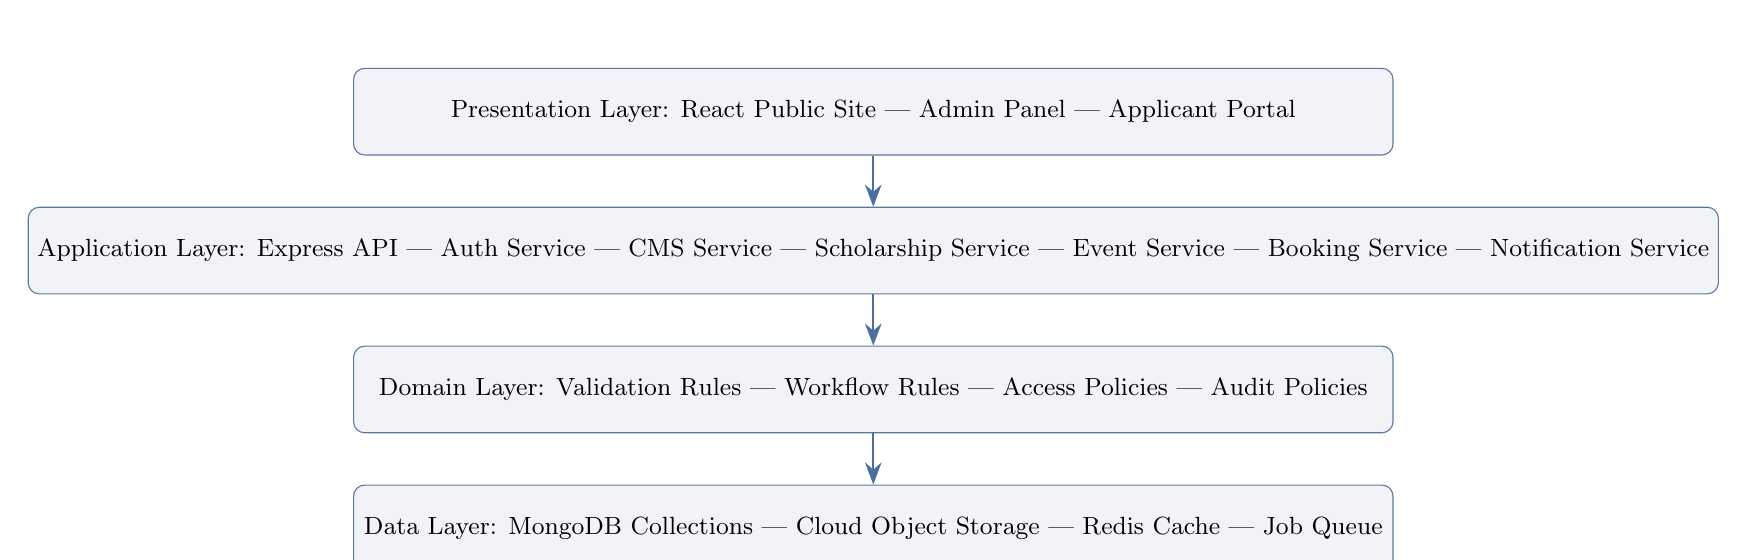
\begin{tikzpicture}[
  box/.style={rectangle, rounded corners=4pt, draw=headerblue!70, fill=headerblue!6, minimum width=13.2cm, minimum height=1.1cm, align=center, font=\small},
  arrow/.style={-{Stealth[length=2.8mm]}, thick, draw=headerblue!75}
]
\node[box] (ui) {Presentation Layer: React Public Site | Admin Panel | Applicant Portal};
\node[box, below=0.65cm of ui] (app) {Application Layer: Express API | Auth Service | CMS Service | Scholarship Service | Event Service | Booking Service | Notification Service};
\node[box, below=0.65cm of app] (domain) {Domain Layer: Validation Rules | Workflow Rules | Access Policies | Audit Policies};
\node[box, below=0.65cm of domain] (data) {Data Layer: MongoDB Collections | Cloud Object Storage | Redis Cache | Job Queue};
\draw[arrow] (ui) -- (app);
\draw[arrow] (app) -- (domain);
\draw[arrow] (domain) -- (data);
\end{tikzpicture}%
}
\caption{Layered Logical Architecture}
\label{fig:logical-architecture}
\end{figure}

\subsection{Component Breakdown}
\rowcolors{2}{rowlight}{rowwhite}
\begin{longtable}{@{}L{2.8cm}L{4.2cm}L{3.0cm}L{3.0cm}L{2.8cm}@{}}
\theadrow \thead{Component} & \thead{Responsibility} & \thead{Inputs} & \thead{Outputs} & \thead{Notes} \\
\endhead
CMS Service & Page/news/blog/gallery/contact workflows & Admin commands, media references & Published content, inquiry state updates & Supports bilingual fields \\
Scholarship Service & Categories, notices, applications, review, recipients & Applicant forms, manager decisions & Application records, status history, recipient publication & Duplicate prevention by notice+email \\
Event Service & Events, registration, QR lifecycle, check-in, feedback & Registration forms, QR scans, feedback entries & Registration records, attendance, feedback metrics & QR regeneration logged \\
Booking Service & Venue inventory, request validation, conflict checks, decisions & Booking requests, admin decisions & Booking status, availability windows & Venue lock used during overlap checks \\
Auth/RBAC Service & Login, reset workflow, authorization checks & Credentials, tokens, route context & Session/token outcome, role verdict & Route and service-layer checks \\
Notification Service & In-app + email delivery for key triggers & Domain events, queue jobs & Notification logs, delivery attempts & Async retries with backoff \\
Audit Service & Action traceability & Critical action events & Immutable audit logs & Actor, action, target, timestamp \\
\bottomrule
\end{longtable}
\rowcolors{0}{}{}

\subsection{High-Level Component Diagram (UML)}
\begin{figure}[H]
\centering
\IfFileExists{high_level_component.png}{%
  \includegraphics[width=0.94\textwidth]{high_level_component.png}%
}{%
  \fbox{\begin{minipage}[c][6cm][c]{0.9\textwidth}\centering
  \textbf{Placeholder: High-Level Component Diagram}\\
  \texttt{high\_level\_component.png}
  \end{minipage}}%
}
\caption{UML Component Diagram}
\label{fig:component-diagram}
\end{figure}

\subsection{Key Design Decisions}
\rowcolors{2}{rowlight}{rowwhite}
\begin{longtable}{@{}L{3.0cm}L{4.1cm}L{3.3cm}L{4.8cm}@{}}
\theadrow \thead{Decision} & \thead{Options Considered} & \thead{Chosen Option} & \thead{Reason} \\
\endhead
Application architecture & Monolith, modular monolith, microservices & Modular monolith with service boundaries & Best balance for current team size; supports gradual extraction \\
Web stack & MERN, Laravel, Django & MERN (React + Node/Express + MongoDB) & Team alignment and faster full-stack iteration \\
Asynchronous processing & In-process jobs, DB polling, Redis queue & Redis + BullMQ & Reliable retries and decoupled side effects \\
Media handling & Local filesystem, DB blobs, object storage & Object storage (Cloudinary/S3) & Better scalability and delivery performance \\
Booking concurrency & Best-effort check, optimistic only, lock-based validation & Lock-based validation around overlap check & Prevents race-condition double booking \\
Notification model & Synchronous send, asynchronous queue & Asynchronous queue with retries & Core transactions stay responsive under transient failures \\
\bottomrule
\end{longtable}
\rowcolors{0}{}{}

\section{Data Design}

\textbf{Core Entities}
Page, NewsPost, GalleryAlbum, MediaItem, ContactInquiry, ScholarshipCategory, ScholarshipNotice, ScholarshipApplication, ScholarshipUpdate, RecipientPublication, Event, EventRegistration, EventFeedback, Venue, VenueBooking, User, NotificationLog, and AuditLog.

\textbf{Key Relationships}
\begin{itemize}[nosep]
\item ScholarshipNotice $\rightarrow$ ScholarshipApplication (1:N)
\item Event $\rightarrow$ EventRegistration (1:N)
\item EventRegistration $\rightarrow$ EventFeedback (1:0..1)
\item Venue $\rightarrow$ VenueBooking (1:N)
\item User $\rightarrow$ NotificationLog/AuditLog (1:N)
\end{itemize}

\textbf{Constraints (Unique, Nullability, Validation)}
\begin{itemize}[nosep]
\item Unique identity and route constraints, including user email and page slug.
\item Duplicate prevention constraints for scholarship applications and event registrations.
\item QR token uniqueness and one-feedback-per-registration constraints.
\item Venue-booking overlap validation for active booking states.
\end{itemize}

\textbf{Data Lifecycle Notes}
\begin{itemize}[nosep]
\item Content uses publish-state lifecycle (Draft, Review, Published).
\item Scholarship and booking records maintain status-history oriented transitions.
\item Notification and audit records are append-oriented for traceability.
\item Media/document binaries are stored in object storage; metadata is stored in MongoDB.
\end{itemize}

\subsection{Logical Data Model}
The data model is organized around module-specific aggregates that share common identity, notification, and audit services. The design below reflects the current project scope without introducing extra business entities.

\rowcolors{2}{rowlight}{rowwhite}
\begin{longtable}{@{}L{3.4cm}L{5.0cm}L{5.3cm}@{}}
\theadrow \thead{Entity} & \thead{Purpose} & \thead{Key Fields / Notes} \\
\endhead
Page & Public CMS content page & slug, titles and bodies in Bangla/English, template, status, SEO metadata. \\
NewsPost & News or blog entry & type, title, body, category, tags, cover image, scheduled publish time. \\
GalleryAlbum & Group of media assets & name, description, visibility, and publication status. \\
MediaItem & Uploaded image or video & filename, MIME type, storage path, size, album reference, uploader. \\
ContactInquiry & Public contact submission & name, email, subject, message, status, created time, admin response trail. \\
ScholarshipCategory & Scholarship definition bucket & name, amount type, amount, description, and display order. \\
ScholarshipNotice & Public scholarship announcement & category, title, eligibility, open/close dates, deadline, status. \\
ScholarshipApplication & Applicant submission & notice reference, applicant identity, form data, attachment path, status history. \\
ScholarshipUpdate & Follow-up announcement for a notice & notice reference, update title, content, published time. \\
RecipientPublication & Awarded recipient list record & notice reference, applicant reference, publication timestamp. \\
Event & Public departmental event & bilingual title, description, venue, start/end time, capacity, registration deadline. \\
EventRegistration & Event sign-up record & event reference, attendee identity, QR token, check-in timestamp. \\
EventFeedback & Post-event feedback submission & event reference, registration reference, rating, comments. \\
Venue & Bookable room or space & name, type, capacity, equipment, active status. \\
VenueBooking & Booking request and decision record & venue reference, requester, start/end time, purpose, status, comment. \\
User & Administrative or applicant account & name, email, password hash, role, status, session state. \\
NotificationLog & Notification trail & user reference, trigger event, channel, delivery status, sent time. \\
AuditLog & Administrative action history & actor, action, target type/id, timestamp, optional metadata. \\
\bottomrule
\end{longtable}
\rowcolors{0}{}{}

\subsection{Critical Constraints and Indexes}
\rowcolors{2}{rowlight}{rowwhite}
\begin{longtable}{@{}L{4.2cm}L{5.5cm}L{5.2cm}@{}}
\theadrow \thead{Entity} & \thead{Constraint / Index} & \thead{Design Rationale} \\
\endhead
User & UNIQUE(email) & Prevent duplicate identities \\
Page & UNIQUE(slug) & Stable public routing \\
NewsPost & INDEX(type, publish\_at DESC) & Fast public listing and scheduled publishing \\
GalleryAlbum & UNIQUE(name) & Prevent duplicate album names in admin workflow \\
MediaItem & INDEX(album\_id, uploaded\_by) & Efficient album rendering and ownership lookup \\
ContactInquiry & INDEX(status, created\_at DESC) & Fast inbox triage for administrators \\
ScholarshipCategory & UNIQUE(name) & Prevent duplicate scholarship buckets \\
ScholarshipApplication & UNIQUE(notice\_id, applicant\_email) & Duplicate prevention \\
ScholarshipUpdate & INDEX(notice\_id, published\_at DESC) & Chronological scholarship notice updates \\
RecipientPublication & UNIQUE(notice\_id, applicant\_id) & One publication entry per awarded applicant \\
EventRegistration & UNIQUE(event\_id, email) & One registration per participant/event \\
EventRegistration & UNIQUE(qr\_token) & QR token uniqueness \\
EventFeedback & UNIQUE(registration\_id) & One feedback response per attendee registration \\
Venue & UNIQUE(name, type) & Keep venue inventory consistent \\
VenueBooking & INDEX(venue\_id, status, start\_at, end\_at) & Fast conflict checks for active slots \\
NotificationLog & INDEX(user\_id, channel, sent\_at DESC) & Efficient inbox retrieval by channel \\
AuditLog & INDEX(actor\_id, timestamp DESC) & Actor-centric traceability \\
\bottomrule
\end{longtable}
\rowcolors{0}{}{}

\section{Core Flow Design}
Documented below are two critical end-to-end flows.

\subsection{Flow 1: Scholarship Application Submission}
\textbf{Trigger}: Applicant submits a scholarship application form for an open notice.

\textbf{Steps}
\begin{enumerate}[nosep]
\item Applicant opens an active scholarship notice and fills required fields.
\item System validates payload, checks duplicate constraints, and stores application as Pending.
\item System emits notification event and records audit trail.
\end{enumerate}

\textbf{Success Outcome}: Application is persisted with status history and confirmation is returned.

\textbf{Failure/Edge Cases}
\begin{itemize}[nosep]
\item Duplicate submission attempt is rejected.
\item Closed notice window rejects new submissions.
\item Notification dispatch failure does not roll back committed application.
\end{itemize}

\begin{figure}[H]
\centering
\IfFileExists{activity.png}{%
  \includegraphics[width=0.63\textwidth]{activity.png}%
}{%
  \fbox{\begin{minipage}[c][6cm][c]{0.9\textwidth}\centering
  \textbf{Placeholder: Activity Diagram}\\
  \texttt{activity.png}
  \end{minipage}}%
}
\caption{Flow 1 Activity Diagram}
\label{fig:activity-scholarship}
\end{figure}

\subsection{Flow 2: Venue Booking Request and Decision}
\textbf{Trigger}: Authorized requester submits a venue booking request.

\textbf{Steps}
\begin{enumerate}[nosep]
\item Requester submits venue, time window, and purpose.
\item System acquires venue-scoped lock, checks overlap against active intervals, and stores Pending request.
\item Venue administrator approves or rejects, and requester receives outcome notification.
\end{enumerate}

\textbf{Success Outcome}: Booking state is updated consistently and availability is refreshed.

\textbf{Failure/Edge Cases}
\begin{itemize}[nosep]
\item Overlapping slot is rejected with conflict detail.
\item Duplicate decision request is idempotently handled.
\item Notification delivery retries asynchronously if channel is temporarily unavailable.
\end{itemize}

\begin{figure}[H]
\centering
\IfFileExists{sequence.png}{%
  \includegraphics[width=0.94\textwidth]{sequence.png}%
}{%
  \fbox{\begin{minipage}[c][6cm][c]{0.9\textwidth}\centering
  \textbf{Placeholder: Sequence Diagram}\\
  \texttt{sequence.png}
  \end{minipage}}%
}
\caption{Flow 2 Sequence Diagram}
\label{fig:sequence-booking}
\end{figure}

\section{Security and Access Design}

\textbf{Authentication Approach}
\begin{itemize}[nosep]
\item Token-based authentication for protected admin and applicant routes.
\item Password reset flow with time-limited and auditable reset events.
\end{itemize}

\textbf{Authorization Model (Roles/Permissions)}
\begin{itemize}[nosep]
\item RBAC enforced at route and service layers.
\item Owner-scoped access for applicant records and restricted privileged operations.
\end{itemize}

\textbf{Sensitive Data Handling}
\begin{itemize}[nosep]
\item Uploaded documents and media validated by type, size, and path rules.
\item Scholarship and booking access constrained by role and ownership checks.
\item Database and storage paths separated from public request payloads.
\end{itemize}

\textbf{Audit/Logging Plan}
\begin{itemize}[nosep]
\item Record actor, action, target, and timestamp for critical operations.
\item Keep notification and delivery logs for operational diagnosis.
\item Preserve security-relevant events for incident review.
\end{itemize}

\section{Implementation Plan}

\textbf{Sprint 1 Completed Features}
\begin{itemize}[nosep]
\item Core architecture and module boundaries defined.
\item CMS, scholarship, events, booking, and platform service designs documented.
\item Initial API contract, data model, and index strategy prepared.
\end{itemize}

\textbf{Pending Features for Sprint 2}
\begin{itemize}[nosep]
\item Implement production-ready queue workers and monitoring dashboards.
\item Complete integration tests for conflict-sensitive booking and QR workflows.
\item Finalize deployment automation and environment-specific configuration.
\end{itemize}

\textbf{Technical Risks}
\begin{itemize}[nosep]
\item Concurrency edge cases in booking and event capacity updates.
\item Queue or email-provider instability during peak workflows.
\item Cross-module coupling if boundaries are not enforced in implementation.
\end{itemize}

\textbf{Mitigation Plan}
\begin{itemize}[nosep]
\item Use lock-based booking validation and idempotent mutation endpoints.
\item Apply retry with exponential backoff for asynchronous delivery.
\item Enforce module interfaces and contract tests between services.
\end{itemize}

\section{Testing Plan (Design Level)}

\textbf{Unit Testing Targets}
\begin{itemize}[nosep]
\item Validation rules, status transition logic, and RBAC decision helpers.
\item QR lifecycle states and duplicate-prevention logic.
\end{itemize}

\textbf{Integration Testing Targets}
\begin{itemize}[nosep]
\item Scholarship submit-review-publish flow.
\item Booking request-decision-notification flow under concurrent requests.
\item Event registration-check-in-feedback chain.
\end{itemize}

\textbf{E2E Testing Targets}
\begin{itemize}[nosep]
\item Public content browsing and bilingual switching.
\item Applicant scholarship tracking workflow.
\item Admin decision workflows for booking and scholarship management.
\end{itemize}

\textbf{Known Hard-to-Test Areas}
\begin{itemize}[nosep]
\item Timing-sensitive concurrency races.
\item External email-provider failure scenarios.
\item Queue backlog behavior under sustained peak load.
\end{itemize}

\section{Appendix: Supporting Diagrams}

\subsection*{Use Case Diagram}
\begin{figure}[H]
\centering
\IfFileExists{use_case.png}{%
  \includegraphics[width=0.7\textwidth]{use_case.png}%
}{%
  \fbox{\begin{minipage}[c][6cm][c]{0.7\textwidth}\centering
  \textbf{Placeholder: Use Case Diagram}\\
  \texttt{use\_case.png}
  \end{minipage}}%
}
\caption{UML Use Case Diagram}
\label{fig:use-case}
\end{figure}

\subsection*{UML Class Diagram}
\begin{figure}[H]
\centering
\IfFileExists{uml.png}{%
  \includegraphics[width=\textwidth]{uml.png}%
}{%
  \fbox{\begin{minipage}[c][6cm][c]{0.9\textwidth}\centering
  \textbf{Placeholder: UML Class Diagram}\\
  \texttt{uml.png}
  \end{minipage}}%
}
\caption{UML Domain/Class Diagram}
\label{fig:class-diagram}
\end{figure}

\section{Conclusion}
This System Design Document defines the implementation architecture, component responsibilities, data model, core workflow behavior, security controls, and delivery plan for the Digital Department Hub. The design is structured for immediate Sprint 2 execution with clear module boundaries, test targets, and risk controls suitable for Lab 4 evaluation and engineering handoff.

\end{document}
